\documentclass{beamer}

\mode<presentation> 
{
    \usetheme{Madrid}
}

\usepackage[utf8x]{inputenc}
\usepackage[english,russian]{babel}
\usepackage[T2A]{fontenc}
\usepackage{graphicx}
\usepackage{booktabs} 
\usepackage{mathtools}
\usepackage{amsmath}
\usepackage{wasysym}
\usepackage{subfig}
\usepackage{hyperref}
\usepackage{ulem}
\usepackage{ragged2e}
\usepackage{algorithm2e}
\usepackage{minted}


\DeclarePairedDelimiter\ceil{\lceil}{\rceil}
\DeclarePairedDelimiter\floor{\lfloor}{\rfloor}


\usemintedstyle{borland}

\usefonttheme[onlymath]{serif}

\hypersetup
{
    colorlinks=true,
    linkcolor=white, 
    urlcolor=cyan
}

\title[Лекция 6]
{
    Лекция 6: Рекусивные структуры данных и динамическая память в языке Си
} 


\author[Д. А. Караваев]{Д. А. Караваев}

\institute[СПбГУТ] 
{
    Санкт-Петербургский государственный университет телекоммуникаций \\ им. проф. М. А. Бонч-Бруевича \\ 
    \vspace{0.2cm}
    Факультет РТС, Кафедра РОС \\
    \vspace{0.2cm}
    Факультатив <<Программирование в ЦОС>> \\
    \vspace{0.2cm}
    Осень 2019
}

\date[25.11.2019]{25.11.2019 Санкт-Петербург} 

\begin{document}
    \begin{frame}
        \titlepage 
    \end{frame}
    \begin{frame}[fragile]
        \frametitle{Cвязные списки}
        \justifying
        Простейшим примером {\it рекурсивной} структурой данных является {\bf однонаправленный связаный список}, который состоит из {\it головы} и {\it хвоста}, который также является связным списком, либо отсутствует.
        \begin{figure}[!tbp]
           \centering
           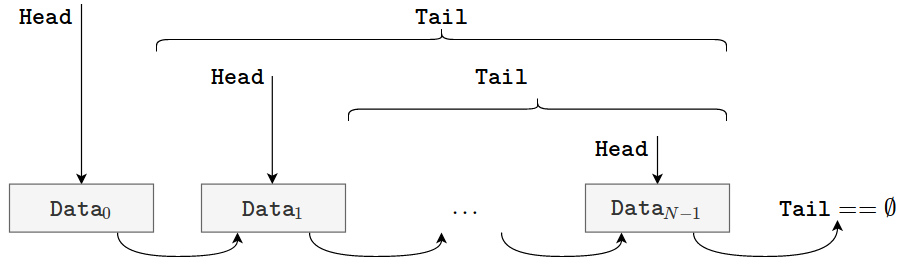
\includegraphics[width=\textwidth]{pics/forward_list.png}
        \end{figure}
    \end{frame}
    \begin{frame}[fragile]
        \frametitle{Реализация в язык Си}
        \justifying
        Односвязный список можно реализовать через структуру, в которой содержится {\it указатель} на хвост.
        \begin{minted}[frame=lines,         framesep=2mm,
                       baselinestretch=1.2, fontsize=\footnotesize,
                       linenos]{c}
/* Определение списка: */
typedef struct list_impl 
{
    int data; /* Содержимое головы. */
    struct list_impl* tail; /* Хвост. */
} list_impl_t;
/* Создание головы: */
list_impl_t head = {.data = 100, .tail = NULL}; /* Нулевой указатель! */
/* Создание хвоста: */
list_impl_t tail = {.data = 200, .tail = NULL};
/* Добавление хвоста: */
head.tail = &tail; 
        \end{minted}
    \end{frame}
    \begin{frame}[fragile]
        \frametitle{Инкапсуляция работы со списком}
        \justifying
        \begin{minted}[frame=lines,         framesep=2mm,
                       baselinestretch=1.2, fontsize=\footnotesize,
                       linenos]{c}
/* Управляющяя структура с головой списка (Данные): */
typedef struct 
{
    list_impl_t* head; /* Хвост. */
    size_t       size;  /* Число элементов в списке. */
} list_t;
/* Методы: */
/* Добавить элемент в конец списка: */
void list_emplace_back(list_t* list, int data);
/* Подсчитать число элементов в списке с данным значением: */
size_t list_count(const list_t* list, int data);
/* Узнать значения по индексу: */
int list_at(const list_t* list, size_t index);
/* Удалить элемент из списка по индексу: */
void list_delete(list_t* list, size_t index);
        \end{minted}
    \end{frame}
    \begin{frame}[fragile]
        \frametitle{Двунаправленный связный список}
        \justifying
        \begin{minted}[frame=lines,         framesep=2mm,
                       baselinestretch=1.2, fontsize=\footnotesize,
                       linenos]{c}
typedef struct list_impl 
{
    int data; /* Содержимое головы. */
    struct list_impl* succ; /* Последующий элемент. */
    struct list_impl* pred; /* Предыдущий элемент. */
} list_impl_t;
/* Создание списка: */
list_impl_t first = {.data = 100, .succ = NULL, .pred = NULL};
list_impl_t second = {.data = 200, .succ = NULL, .pred = &first};
first.succ = &second;
        \end{minted}
        \begin{figure}[!tbp]
           \centering
           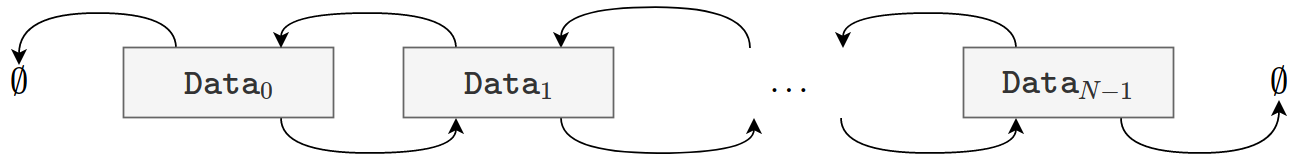
\includegraphics[width=\textwidth]{pics/list.png}
        \end{figure}
    \end{frame}
    \begin{frame}[fragile]
        \frametitle{Замечания по поводу работы со списками}
        \begin{enumerate}
            \justifying
            \item {\bf Алгоритмическая сложность}: Большинство операций в списках имеют $O(N)$ или $\Theta(N)$ временную сложность;
            \item {\bf Реализация стека и очереди}: Списки удобно использовать для реализации стека (или очереди), так как число элементов не ограничено;
            \item {\bf Операции над двунаправленном списком}: Можно опредлить большое множество полезных операций над двунаправленном списком.
            \item {\bf Хранения "тяжелых"\ структур}: Списки удобны для хранения структур (пользовательских типов) с большим количеством полей, к которым нет необходимости применять индексацию.
        \end{enumerate}
    \end{frame}
    \begin{frame}[fragile]
        \frametitle{Дерево бинарного поиска}
        \justifying
        Другим примером рекурсивной структуры данных служит {\bf дерево}, которое состоит из {\bf корня} (родителя), в котором хранится значение ({\it ключ}) и у которого может быть несколько {\bf поддеревьев} (потомков). Деревья, у которых нет поддеревьев, называются {\bf листьям}.
        \par
        \vspace{0.5cm}
        \justifying
        Если у дерева может быть не более двух поддеревьев, и {\it для каждого родительского ключа ключи большее него храняться в правом поддереве, а меньше в левом}, то таком дерево называется {\bf дерево бинарного поиска}. В нашем случае, все значения в дереве {\it уникальны}.
    \end{frame}
    \begin{frame}[fragile]
        \frametitle{Иллюстрация дерева бинарного поиска}
        \begin{figure}[!tbp]
           \centering
           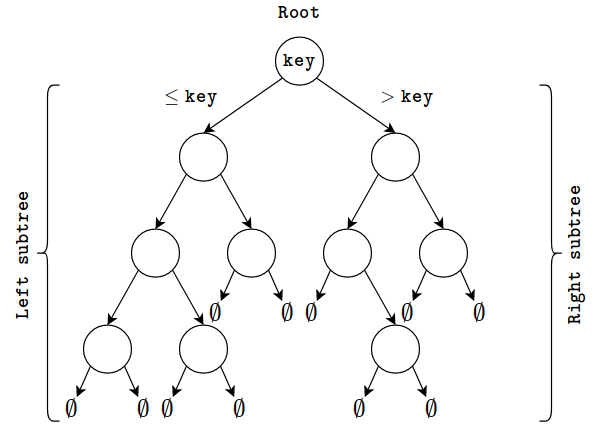
\includegraphics[width=0.85\textwidth]{pics/tree.png}
        \end{figure}
    \end{frame}
    \begin{frame}[fragile]
        \frametitle{Представление дерева бинарного поиска в языке Си}
        \begin{minted}[frame=lines,         framesep=2mm,
                       baselinestretch=1.2, fontsize=\footnotesize,
                       linenos]{c}
typedef struct bstree_node
{
    int key; /* Ключ. */
    struct bstree_node* left; /* Левое поддерево. */
    struct bstree_node* rigth; /* Правое поддерево. */
} bstree_node_t;
/* Управляющяя структура с корнем дерева: */
typedef 
{
    bstree_node_t* root; /* Корень дерева. */
    size_t size; /* Размер дерева. */
} bstree_t;
void bstree_emplace(bstree_t* tree, int key); /* Добавить элемент. */
int bstree_find(const bstree_t* tree, int key); /* Найти элемент. */
void bstree_delete(bstree_t* tree, int key); /* Удалить элемент. */
        \end{minted}
    \end{frame}
    \begin{frame}[fragile]
        \frametitle{Замечания к дереву бинарного поиска}
        \begin{enumerate}
            \justifying
            \item {\bf Алгоритмическая сложность}:
            Когда, дерево заполнено равномерно алгоритмеческая сложность всех операций пропорциональна его выcоте $O(h) = O(\log N)$, где $N$ - число элементов в дереве.
            \item {\bf Расбаланисровка}:
            Яление, при котором основная "масса"\ элементов дерева сосредоточена вдоль одного края. Тогда дерево {\it вырождается} в однонаправленный список и преимущество в скорости поиска элементов теряется. Для борьбы с этим явлением используют более сложные реализации бинарных деревьев (красно-черные и AVL деревья).
            \item {\bf Ассоциативный контейнер}:
            Деревья часто используются для реализации {\it ассоциативного контейнера (словарь)}, в котором тип индекса ({\it ключа}) может быть любым упорядоченным типом.
        \end{enumerate}
    \end{frame}
    \begin{frame}[fragile]
        \frametitle{Иллюстрация расбалансировки}
        \begin{figure}[!tbp]
           \centering
           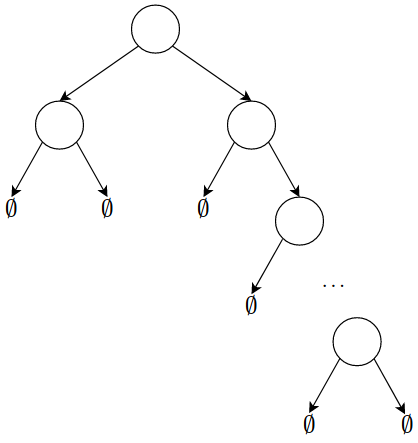
\includegraphics[width=0.6\textwidth]{pics/inbalance.png}
        \end{figure}
    \end{frame}
    \begin{frame}[fragile]
        \frametitle{Реализации вставки в односвязный список}
        \begin{minted}[frame=lines,         framesep=2mm,
                       baselinestretch=1.2, fontsize=\footnotesize,
                       linenos]{c}
void list_emplace_back(list_t* list, int data)
{
    return list_emplace_back_impl(list->head, data);
}
void list_emplace_back_impl(list_impl_t* head, int data)
{
    if (head->tail == NULL)
    {
        list_impl_t tail = {.data = data, .tail = NULL};
        head->tail = &tail; /* Ошибка. tail - локальная переменная! */
        return;
    }

    return list_emplace_back_impl(head->tail, data);
}
        \end{minted}
    \end{frame}
    \begin{frame}
        \begin{center}
        \baselineskip 20.0mm
        \Huge Спасибо за внимание!
        \end{center}
    \end{frame}
\end{document}
